\documentclass[10pt,letterpaper]{article}
\usepackage[spanish]{babel}
\usepackage{listings}
\usepackage{graphicx} %paqute para que pueda jalar mi imagen del diagrama
\usepackage{float}
\usepackage{comment}%para comentar desde la pergunta 11 a la 15
% Preámbulo

\title{Análisis de ingeniería inversa sobre un sistema \textit{legacy}}
\author{Base de Datos }
\date{\today}

\usepackage{xcolor}

\definecolor{codegreen}{rgb}{0,0.6,0}
\definecolor{codegray}{rgb}{0.5,0.5,0.5}
\definecolor{codepurple}{rgb}{0.58,0,0.82}
\definecolor{backcolour}{rgb}{0.95,0.95,0.92}

\lstdefinestyle{mystyle}{
    backgroundcolor=\color{backcolour},   
    commentstyle=\color{codegreen},
    keywordstyle=\color{magenta},
    numberstyle=\tiny\color{codegray},
    stringstyle=\color{codepurple},
    basicstyle=\ttfamily\footnotesize,
    breakatwhitespace=false,         
    breaklines=true,                 
    captionpos=b,                    
    keepspaces=true,                 
    numbers=left,                    
    numbersep=5pt,                  
    showspaces=false,                
    showstringspaces=false,
    showtabs=false,                  
    tabsize=2
}
\lstset{style=mystyle}

 

\begin{document}
\maketitle




\section{Introducción}
Se nos ha encomendado realizar ingenria inversa y posteriormente el analisis de un conjunto de archivos que comprenden
la definicion estructural y logica de la Base de Datos de un sistema "Legacy".Con la finalidad de practicar e integrar todo lo 
aprendido 
\section{Descripción del problema}
Lo que hace este programa en SQL , es como un archivero digital para organizar los datos 
de una escuela,y que todo este donde debe de estar ya que crea diferentes listas que se
conectan entre si para guardar la informacion bien estructurada y limpia.
\section{Análisis}
Pero ,¿Qué es lo que hace exactamente ?
Bueno en primer lugar tenemos que crear un espacio inicial donde se va a guardar todo 
\begin{table}[h!]%para que lo ponga justo abajo de "Analisis"
    \begin{tabular}{| c |p{10cm} |} %esto srive para dar un salto de linea para que no se siga de largo LaTex
        \hline
        TABLAS & ¿QUE ORGANIZA? \\
        \hline
        Departamentos y Profesores & Hace una lista de las areas de la escuela
                                    y registra a los profesores identificando a que 
                                    area pertence cada uno\\ \hline
        
        Curos y Aulas              & Registra materias que se imparten , que profesor las imparte
                                     y los salones con disponibilidad y cupo maximo\\ \hline

        Horarios                   & Acomoda el día , a que hora y en que salón toca cada materia\\ \hline
        
        Estudiantes e Inscripciones & Guarda los datos personales de los alumnos y lleva un control de 
                                      las materias que tienen inscritas\\ \hline
        
        Calificaciones                & Crea un espacio exclusivo para guardar las calificaciones finales de los
                                      alumnos en cada materia que tomaron\\ \hline
    \end{tabular}
\end{table}

\section{Diagramas y resultados}
%DER ingeneria inversa
\begin{figure}[H]
    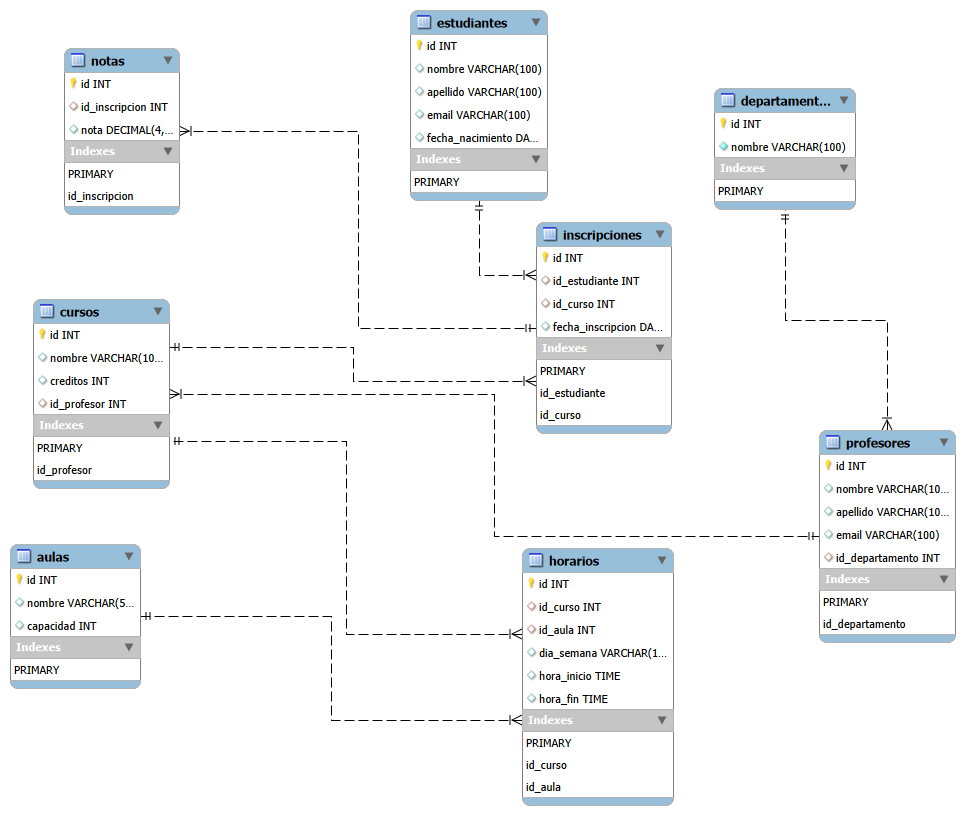
\includegraphics[scale=0.4]{images/Ingeneria-Inversa.png}
    \caption{Diagrama Entidad - Relacion del Sistema}
    \label{fig-Ingeneria-Inversa}
    \end {figure}
\section{Implementación y validación}

%pregunta 1
\begin{figure}[H]
\caption{Implementacion de Cosulta en SQL para la Pregunta 1}
 \includegraphics[width=\textwidth]{images/P1.png}
 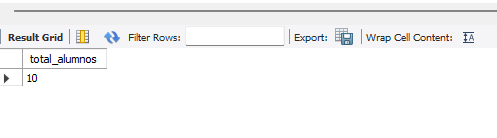
\includegraphics[width=\textwidth]{images/P1.1.png}
  \section*{ ¿Cuales son los estudiantes inscritos en el curso de Algebra?}
  Lo que tuve que hacer fue poner el select busca a todos los alumnos
   , luego se va  a la tabla de inscripciones, después busca con un Join
    los cursos que tengan inscripciones, $id\_curso$,y para finalizar 
    busca el nombre del curso que en este caso es Álgebra.

\end{figure}

%Pregunta 2 
\section*{}
\begin{figure}[H]
 \graphicspath{{images/}}
 \caption{Implementacion de Consulta en SQL para la Pregunta 2}
\includegraphics[width=\textwidth]{P2.png}
  \section*{¿Que cursos imparte el Profesor Martinez?}
  Programacion , de igual manera ocupamos el JOIN para conectarnos a la 
  tabla de cursos con la de profesores con el ON es como un puente que 
  une los datos con el ID del profesor
\end{figure}

%pregunta 3 
\section*{}
\begin{figure}[H]
    \graphicspath{{images/}}
    \caption{Implementación de Consulta en SQL para la Pregunta 3}
    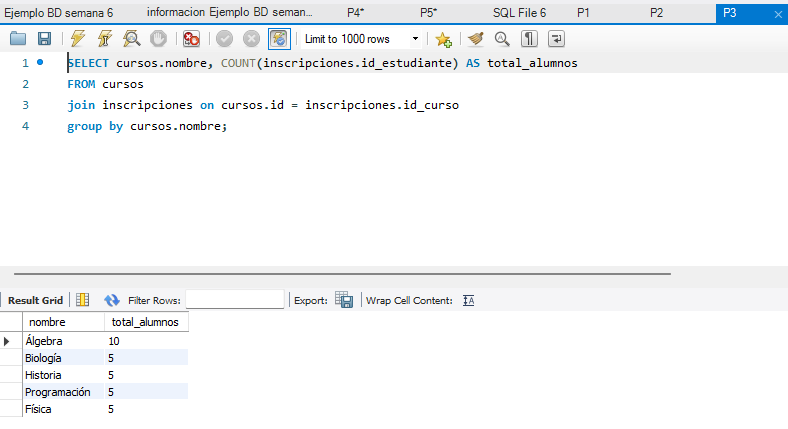
\includegraphics[width=\textwidth]{P3.png}
    \section*{¿Cuantos estudiantes estan inscritos en cada curso?}
 Algerbra = 6, Biologia = 3 , Historia = 3, Programacion = 3 , Fisica = 3
 ocupe un Count , que es un contador , que le dice a la BD que sume todos 
 los alumnos, y el GRUOP BY es la que ordena a la BD qeu agrupe todos los 
 resultados guiandose por el nombre de la materia 
    

\end{figure}

%pregunta 4
\section*{}
\begin{figure}[H]
    \graphicspath{{images/}}
    \caption{Implementación de Consulta en SQL para la Pregunta 4}
    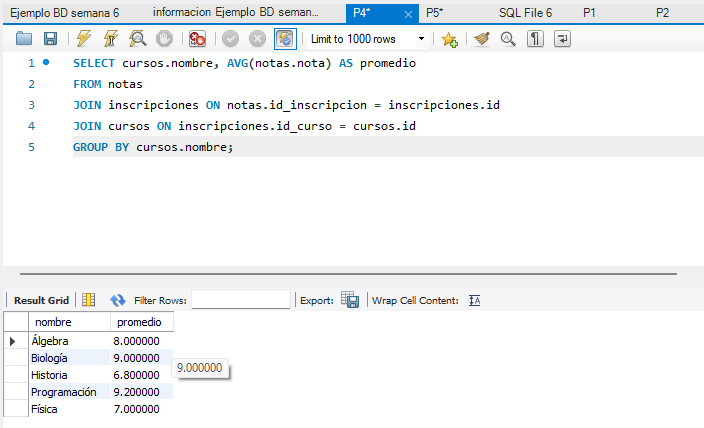
\includegraphics[width=\textwidth]{P4.png}
    \section*{¿Cual es el promedio de notas por curso? }
    Biologia con un promedio de 9.0 ponemos un select dec cursos.nombre
  y ponems un nueva funcion AVG (notas.nota) que le dice a BD queire el 
  promedio de las notas de la tabala de notas  pero hazlas como Promedio 
 hace 2 JOIN que revisa cursos  e  inscripciones y los agrupa por Cursos.nombre
    
\end{figure}

%pregunta 5
\section*{}
\begin{figure}[H]
    \graphicspath{{images/}}
    \caption{Implementación de Consulta en SQL para la Pregunta 5}
    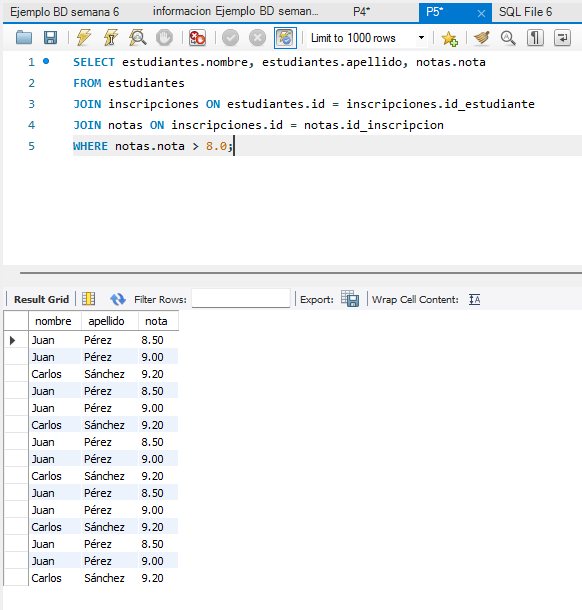
\includegraphics[width=\textwidth]{P5.png}
    \section*{¿Qué lista de estudiantes tiene notas mayores a 8.0?}
Juan	Pérez	8.50
Juan	Pérez	9.00
Carlos	Sánchez	9.20
Juan	Pérez	8.50
Juan	Pérez	9.00
Carlos	Sánchez	9.20
Juan	Pérez	8.50
Juan	Pérez	9.00
Carlos	Sánchez	9.20

hacemos nuevamente un select que pida  nombre , apellidos y notas de todos los alumnos inscritos
 a un curso , luego hacemos unos JOINS , el primero pide las inscripciones x estudiante y que devuelva
  las inscripcones con el id de estudainte , el segundo las notas de las inscripciones (id) y un where 
  donde se estipule que las solamente nos de los estudaintes con las notas mayores a 8.0
    
\end{figure}

%pregunta 6
\section*{}
\begin{figure}[H]
    \graphicspath{{images/}}
    \caption{Implementación de Consulta en SQL para la Pregunta 6}
    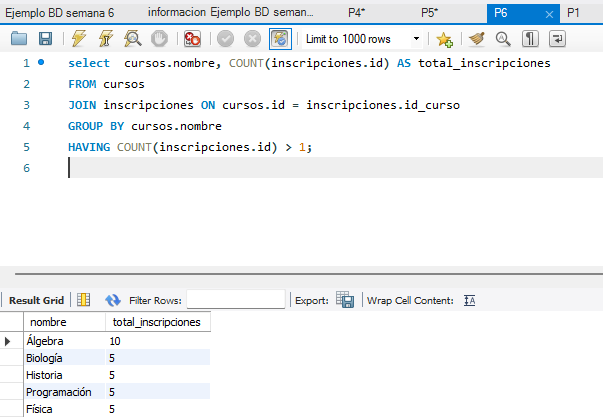
\includegraphics[width=\textwidth]{P6.png}
    \section*{¿Que cursos tienen mas de una inscripcion?}
\end{figure}

%pregunta 7
\section*{}
\begin{figure}[H]
    \graphicspath{{images/}}
    \caption{Implementación de Consulta en SQL para la Pregunta 6}
    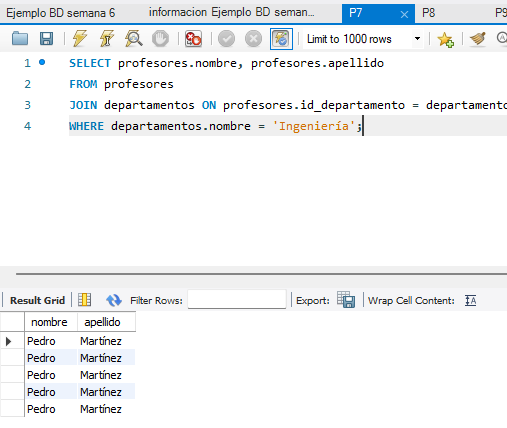
\includegraphics[width=\textwidth]{P7.png}  
    \section*{¿Que profesores pertenecen al departamento de Ingeneria?}
\end{figure}

%pregunta 8
\section*{}
\begin{figure}[H]
    \graphicspath{{images/}}
    \caption{Implementación de Consulta en SQL para la Pregunta 6}
    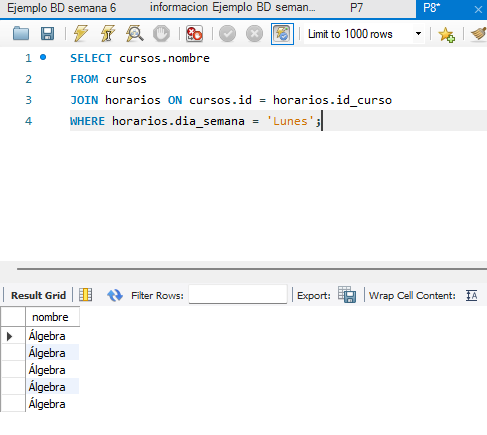
\includegraphics[width=\textwidth]{P8.png}  
    \section*{¿Cuales son los cursos  programados los Lunes?}
\end{figure}

%pregunta 9
\section*{}
\begin{figure}[H]
    \graphicspath{{images/}}
    \caption{Implementación de Consulta en SQL para la Pregunta 6}
    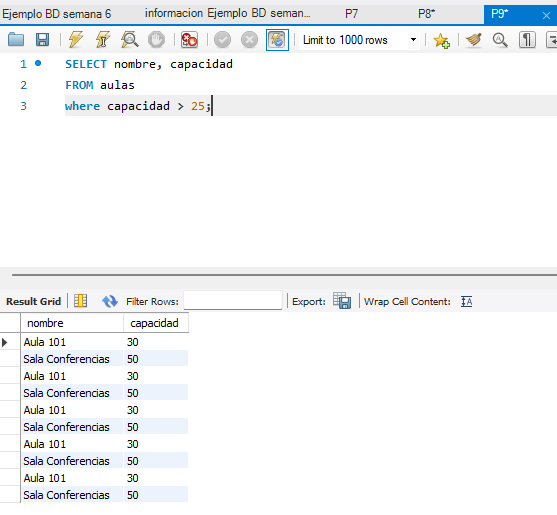
\includegraphics[width=\textwidth]{P9.png}
    \section*{¿Que aulas tienen una capacidad mayor a 25?}
\end{figure}

%pregunta 10
\section*{}
\begin{figure}[H]
    \graphicspath{{images/}}
    \caption{Implementación de Consulta en SQL para la Pregunta 6}
    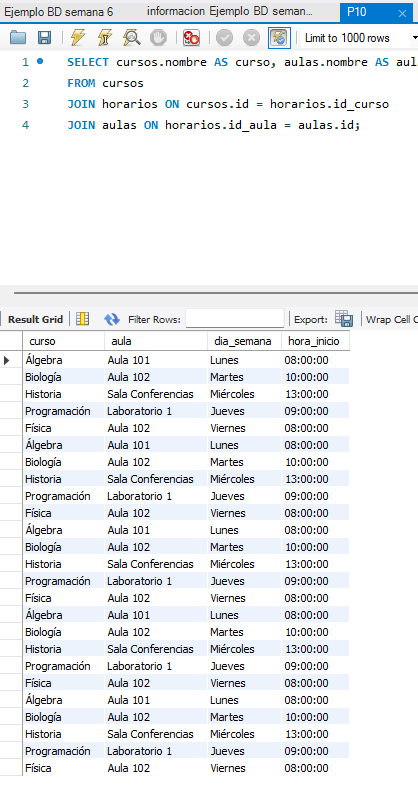
\includegraphics[width=\textwidth]{P10.png} %cambiar esto 
    \section*{¿Que aulas tienen una capacidad mayor a 25?}
    
\end{figure}

\begin{comment}
%pregunta 11
\section*{}
\begin{figure}[H]
\graphicspath{{images/}}
\caption{Implementación de Consulta en SQL para la Pregunta 6}
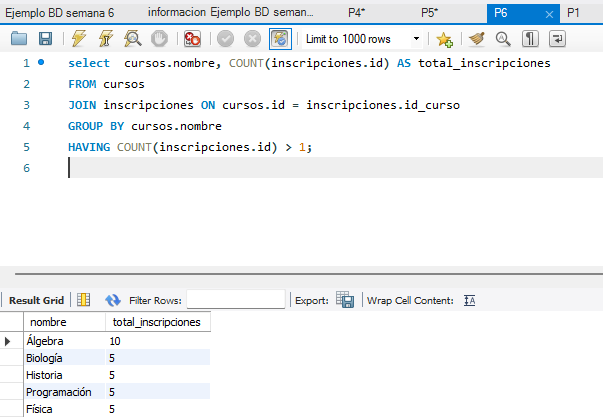
\includegraphics[width=\textwidth]{P6.png} %cambiar esto 
\section*{Lista de cursos con su aula y horario}

\end{figure}

%pregunta 12
\section*{}
\begin{figure}[H]
\graphicspath{{images/}}
\caption{Implementación de Consulta en SQL para la Pregunta 6}
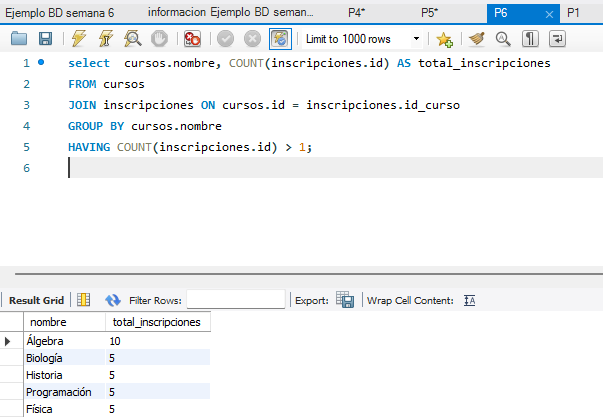
\includegraphics[width=\textwidth]{P6.png} %cambiar esto 
\section*{¿Cuantos profesores hay por departamento?}

\end{figure}

%pregunta 13
\section*{}
\begin{figure}[H]
\graphicspath{{images/}}
\caption{Implementación de Consulta en SQL para la Pregunta 6}
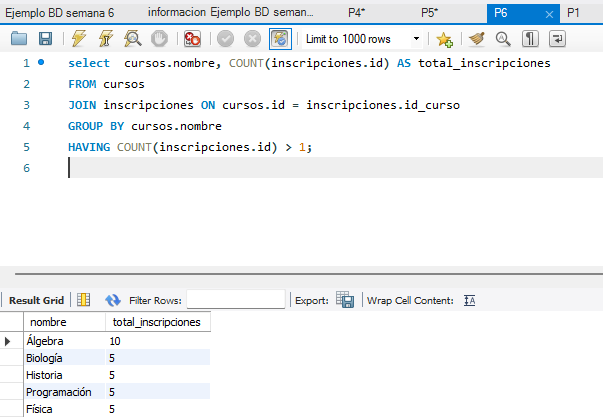
\includegraphics[width=\textwidth]{P6.png} %cambiar esto 
\section*{¿Cuantos profesores hay por departamento?}

\end{figure}

%pregunta 14
\section*{}
\begin{figure}[H]
\graphicspath{{images/}}
\caption{Implementación de Consulta en SQL para la Pregunta 6}
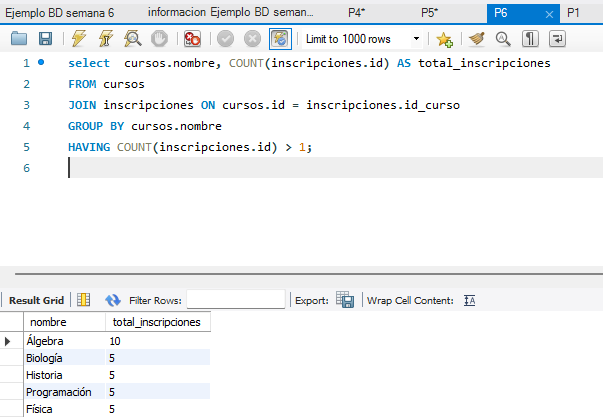
\includegraphics[width=\textwidth]{P6.png} %cambiar esto 
\section*{¿Que cursos no tienen estudiantes inscritos?}

\end{figure}

%pregunta 15
\section*{}
\begin{figure}[H]
\graphicspath{{images/}}
\caption{Implementación de Consulta en SQL para la Pregunta 6}
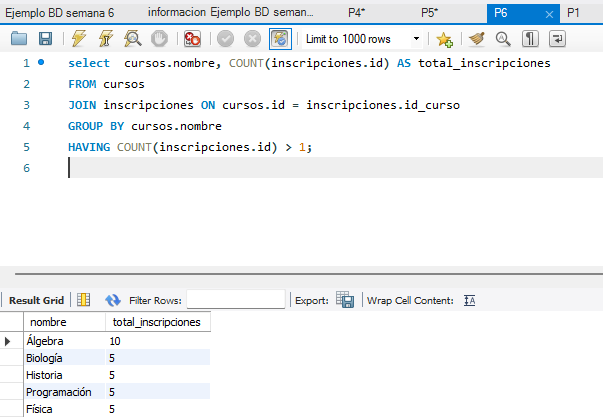
\includegraphics[width=\textwidth]{P6.png} %cambiar esto 
\section*{¿Que estudiantes estan inscritos en mas de un curso?}

\end{figure}
\end{comment}


\section{Conclusiones}
 


\end{document}